\chapter{Design and Development of Airbearing}

An airbearing is just a bearing in which moving surfaces are kept apart by a layer of air. Use of air as a medium creates a near friction less coupling between the mating surfaces. As the detumbling takes place at the orbit, we needed to have a frictionless environment to replicate the actual scenario. The objective was to create a frictionless free to rotate platform for the CubeSat to rest upon.

\subsection{Design and Analysis}

The main part of an airbearing is a porous material which is capable of producing uniform layer of air over which the corresponding mating part can be rested. The porous material selected for our purposes is Graphite (1.7g/cc density).

\begin{figure}[h!]
	\centering
	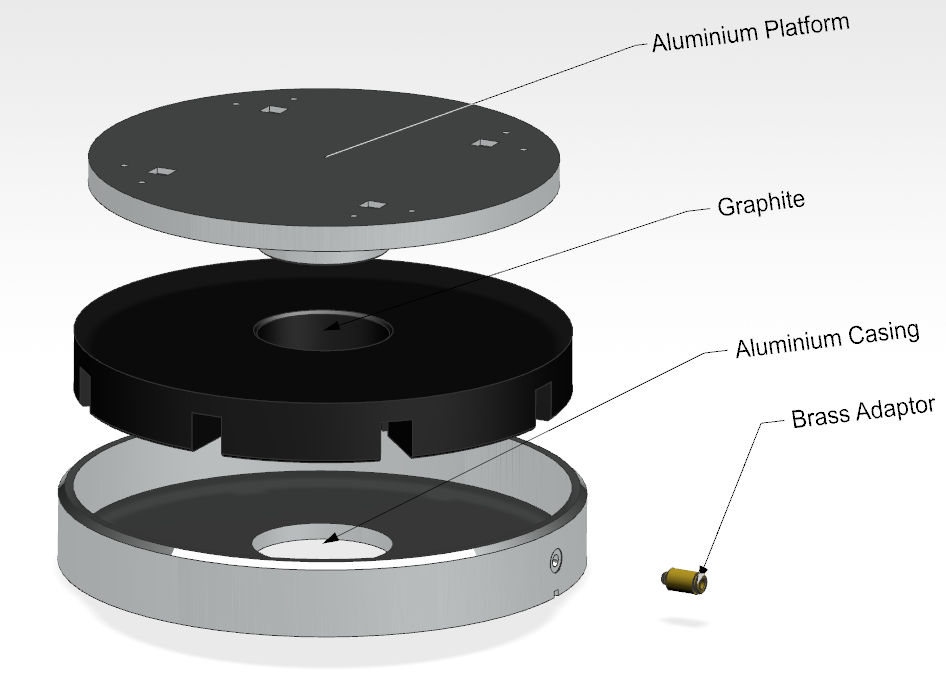
\includegraphics[width=4.5in,height=3.22in]{./images/airBearingStruct.png}
	\caption{Air Bearing}
	\label{fig-air-bearing-struct}
\end{figure}

The platform was made keeping in mind the base area of the CubeSat. A generous amount of 180mm diameter platform was designed for this case. The entire bearing was required to be low profile due to space constraints in the testing rig. A thickness of 25mm of graphite was first chosen to minimise the pressure drop through the graphite while maintaining sufficient stiffness. Air flow channels to allow the pumped air to spread uniformly spread accross the entire graphite, is also designed. The performance of the designed graphite section was analysed on Ansys Fluent.

\noindent Fluid inlet is assigned as the air passages on the graphite. The air compressor that would be used alongside the air bearing was rated 24L capacity. Hence the flow rate from the compressor at 60psi was calculated as follows,\\

\noindent Cubic feet per metre, $CFM = \frac{V\left(P_f - P_i\right)}{14.7t_{fill}}$\\

where, $t_{fill}$ is the fill time to reach 60psi pressure and $V$ is the tank capacity in cubic feet.\\

\noindent Hence the volume flow rate at compressor outlet was calculated to be $0.001088 m^3/s$ From the flow rate the velocity of flow was found and is set as the velocity inlet boundary condition (shown in blue color in \ref{fig-air-bearing-inlet}). The outlet is set to be ambient pressure condition (shown in red color in \ref{fig-air-bearing-outlet}). The porous zone of the graphite is set with the following parameters,\\

\noindent Flow permeability, $k = 1.85\times10^{-15}$ \hspace{160pt}[\ref{flowperm}]

\noindent Viscous resistance, $R = 5.405\times10^{14}$

\noindent Mean diameter of graphite particle, $D_p = 3.16069\times10^{-6}$

\noindent Porosity of graphite, $\epsilon = 0.25$

\noindent Inertial loss coefficient, $C = 5.314\times10^7$ \hspace{140pt}[\ref{inertlosscoeff}]

\vspace{15pt}
\begin{figure}[h!]
	\centering
	\begin{subfigure}[b]{0.45\textwidth}
		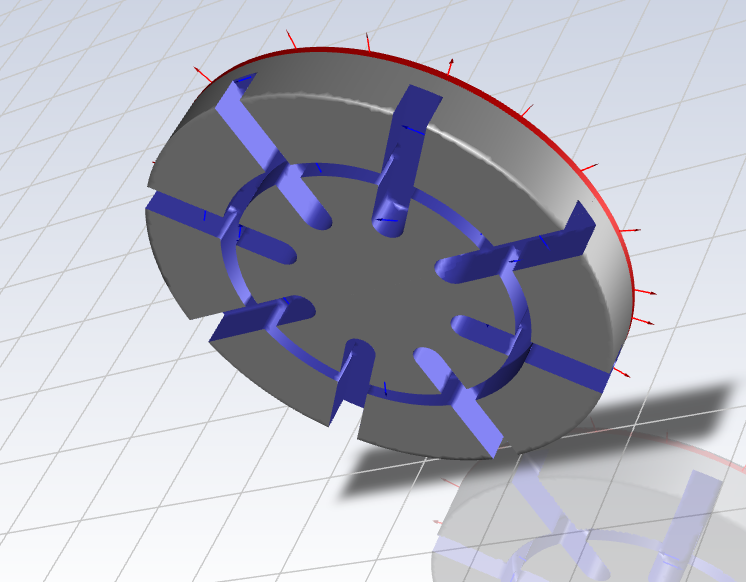
\includegraphics[width=\textwidth,height=2in]{./images/airBearingInlet.png}
		\caption{Velocity inlet}
		\label{fig-air-bearing-inlet}
	\end{subfigure}
	\begin{subfigure}[b]{0.45\textwidth}
		\centering
		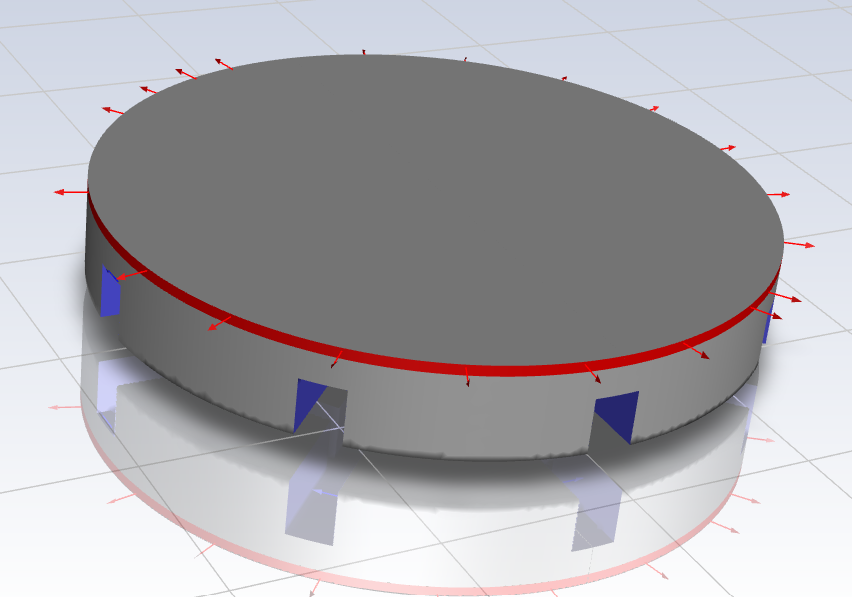
\includegraphics[width=\textwidth,height=2in]{./images/airBearingOutlet.png}
		\caption{Pressure outlet}
		\label{fig-air-bearing-outlet}
	\end{subfigure}
\end{figure}

A density based solver is employed and satidfactory convergence was obtained after about 1000 iterations. The static pressure contour plot of the airflow is shown below.
\pagebreak
 
\begin{figure}[h!]
	\centering
	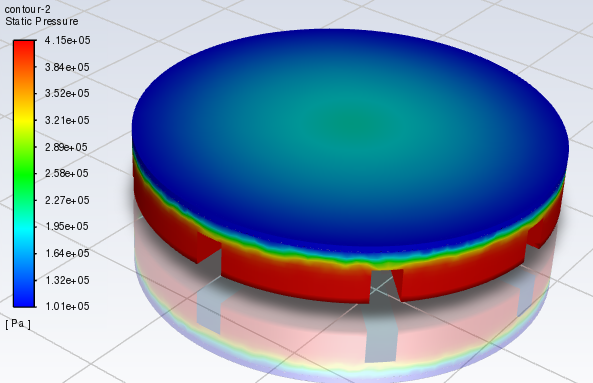
\includegraphics[width=4.5in,height=3.22in]{./images/airBearingAnlsys.png}
	\caption{Pressure contour over the graphite layer}
	\label{fig-air-bearing-anlsys}
\end{figure}

The results shows about 137684 Pa of static pressure on the bearing platform, which translates to 3924 N force. That is about 400 kg lift capacity. This is more than enough for our required application.

\subsection{Fabrication}

\subsubsection{Casing and Platform}

These were fabricated mainly by turning in lathe at 300RPM. A disk shaped Aluminium material of 210x50mm dimensions were turned using orthogonal cutting to yield the platform. A combination of orthogonal cutting, drilling and boring was done on a second piece of the same dimension to obtain the casing. The air inlet hole was machined using a vertical milling machine with a drill size of 8mm. The hole was later tapped with a thread of 1/8BSP, to fasten the tubing adaptor. The air vent groove was machined on the uderside of the casing using a 3mm end mill cutter.

\subsubsection{Graphite}
 
The air flow path on the graphite was machined using a CNC and later sanded manually to obtain better finishing.\\

The graphite was joined together with the casing using an airtight epoxy sealant. The platform is placed over the graphite to yield the finished bearing